\documentclass{article}
\usepackage[margin=1in, paperwidth=8.5in, paperheight=11in]{geometry}
\usepackage{caption}
\usepackage{subcaption}
\usepackage{float}
\usepackage{graphicx}
\usepackage[utf8]{inputenc}
\usepackage[english]{babel}
\usepackage{mathtools}
\usepackage{gensymb}
\usepackage{amstext}
\usepackage{amsmath}
\usepackage{graphicx}
\usepackage{textcomp}
\usepackage{varioref}
\usepackage{fancyref}
\usepackage{subcaption}
\usepackage{comment}
\usepackage{hyperref}
\usepackage{epstopdf}
\usepackage{gensymb}
\usepackage{listings}
\usepackage{xcolor}
\usepackage{listings}
\usepackage{pdfpages}
\usepackage{graphicx}
\usepackage{wrapfig}
\usepackage{lscape}
\usepackage{rotating}
\usepackage{epstopdf}
\usepackage{fancyhdr}
\usepackage{amssymb}
\usepackage{fancyhdr}
\usepackage{soul}
\usepackage{chngcntr}
%font
\usepackage{lmodern} 
\usepackage[sfdefault, light]{roboto}

% Document Setup
\pagenumbering{roman}
\pagestyle{fancy}
\addto\captionsenglish{\renewcommand*\contentsname{Table of Contents}}
\DeclareRobustCommand{\hlr}[1]{{\sethlcolor{red}\hl{#1}}}
\graphicspath{{img/}}
\counterwithin{table}{section} %number tables with section#.table#

\begin{document}

\renewcommand{\headrulewidth}{0pt}
\lhead{Olin College of Engineering, E238}
\chead{}
\rhead{} %\rightmark
\lfoot{2017 Formula SAE Electric}
\cfoot{
\includegraphics[width=3cm]{logo_blue.png}}
\rfoot{\thepage}

\begin{titlepage}

    \centering
    \vfill
    
\includegraphics[width=10cm]{logo_blue.png}

    {\bfseries\Large
        \vskip3cm
        Electrical System Form FSAE-E 2017\\
        Car E238\\
    }

    \begin{table}[H]
        \centering
        \label{my-label}
        \begin{tabular}{lr}
        University Name: & Olin College of Engineering \\ \hline
        Team Name: & Olin Electric Motorsports \\ \hline
        Car Number: & E238 \\ \hline
        ESF Contact: & Alex Hoppe \\ \hline
        e-mail: & Alexander.Hoppe@students.olin.edu \\ \hline
        \end{tabular}
    \end{table}
\vfill

\begin{figure}[H]
\centering
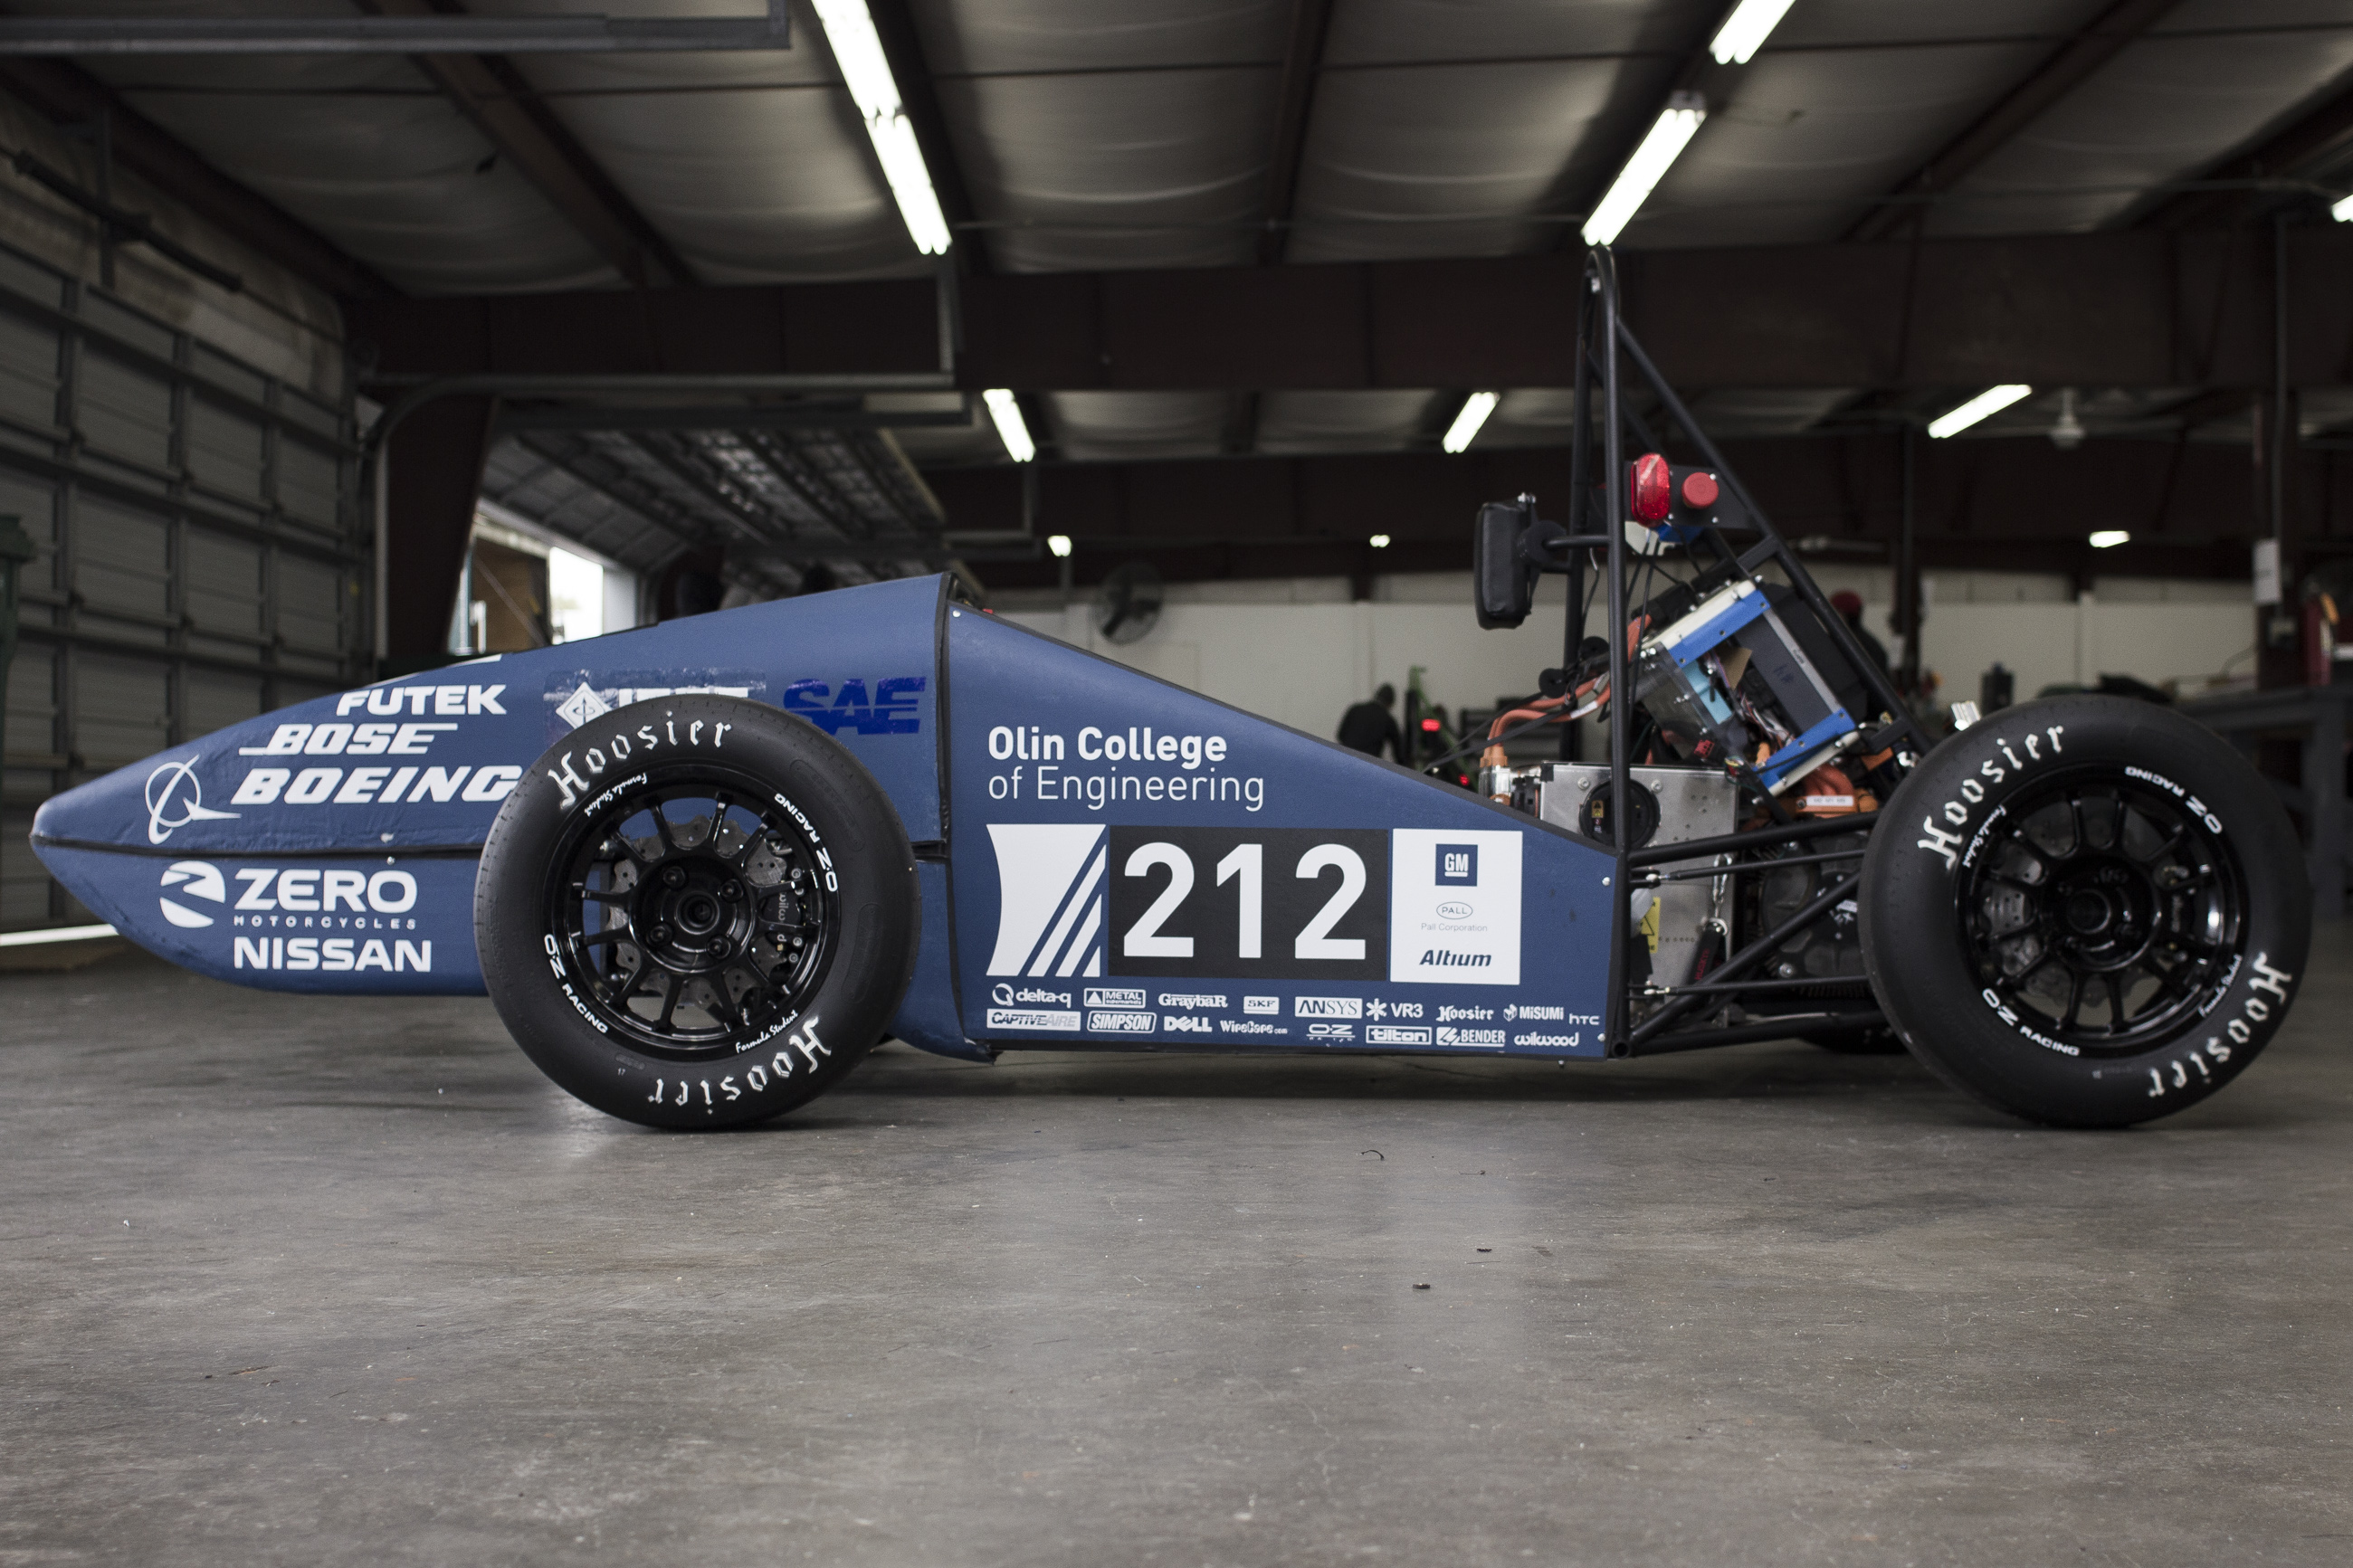
\includegraphics[width = 0.9 \textwidth]{mk1}
\end{figure}

\end{titlepage}

\tableofcontents
\addcontentsline{toc}{section}{Table of Contents}

\newpage
\listoffigures
\addcontentsline{toc}{section}{I List of Figures}

\newpage
\listoftables
\addcontentsline{toc}{section}{II List of Tables}

\newpage
\section*{List of Abbreviations}
\addcontentsline{toc}{section}{III List of Abbreviations}
\begin{itemize}
    \item MSD- Manual Service Disconnect
    \item CONN- Main accumulator connector
\end{itemize}

\setlength{\parindent}{0pt}

\newpage
\pagenumbering{arabic}

\section{System Overview}
	%Short description of the system’s concept 
	%Rough Schematic (blocks) showing all parts affected with the electrical systems and function of the tractive-system
	%No detailed wiring

	\begin{table}[H]
        \centering
        \begin{tabular}{|l|l|}
        \hline
            Maximum Tractive system voltage & 298.8 VDC \\ \hline
            Nominal Tractive system voltage & 266.4 VDC \\ \hline
            Control-system voltage & 12 VDC \\ \hline
            Accumulator configuration & 72s1p \\ \hline
            Total Accumulator capacity & 27 Ah \\ \hline
            Motor type & permanent magnet synchronous motor \\ \hline
            Number of motors & 1 \\ \hline
            Maximum combined motor power in kW & 100 kW \\ \hline
        \end{tabular}
        \caption{General parameters}
        \label{systemtable}
    \end{table}

\section{Electrical Systems}
TODO

\subsection{Shutdown Circuit}

\subsubsection{Description/concept}
%Describe your concept of the shutdown circuit, the master switches, shut down buttons, brake over travel switch, etc.

	\begin{table}[H]
        \centering
        \begin{tabular}{|l|l|}
        \hline
            \textbf{Part} & \textbf{Function} \\ \hline
            GLV Main Switch (GLVMS) & Normally open, with lockout \\ \hline
            Shutdown buttons (SDB) (Left, right, cockpit) & Normally closed \\ \hline
            Brake System Plausibility Device (BSPD) & Normally Open \\ \hline
            Brake over travel switch (BOTS) & Push-pull normally closed button \\ \hline
            Inertia switch & Normally closed \\ \hline
            Battery Management System (AMS) & Normally open \\ \hline
            Insulation Monitoring Device (IMD) & Normally open \\ \hline
            Interlocks & Closed when TS connections are made \\ \hline
            Tractive System Main Switch (SMS) & Normally open, with lockout \\ \hline
        \end{tabular}
        \caption{List of switches in the shutdown circuit}
        \label{switchlist}
    \end{table}

\subsubsection{Wiring / additional circuitry}
%shutdown schematic
TODO

	\begin{table}[H]
        \centering
        \begin{tabular}{|l|l|}
        \hline
            Total Number of AIRs: & 2 \\ \hline
            Current per AIR & 3.9A peak while closing, 0.23A average\\ \hline
            Additional parts consumption within the shutdown circuit: & ??? A TODO: find current of pre/discharge relays \\ \hline
            Total current: & TODO \\ \hline
            Cross sectional area of the wiring used: & 0.00080384 in$^2$ (20 AWG) TODO:spec and convert to mm$^2$ \\ \hline
        \end{tabular}
        \caption{Wiring- Shutdown Circuit}
        \label{ShutdownCircuitTable}
    \end{table}

\subsubsection{Position in car}
%Provide CAD-renderings showing the relevant parts. Mark the parts in the renderings, if necessary.
TODO

\subsection{IMD}
\subsubsection{Description (type, operation parameters)}
%Describe the IMD used and use a table for the common operation parameters, like supply voltage, set point, etc. Also, describe how the IMD indicator light is wired, etc.
TODO

	\begin{table}[H]
	    \centering
	    \begin{tabular}{|l|l|}
	    \hline
	        Supply voltage range: & 10...36VDC \\ \hline
	        Supply voltage & 12VDC \\ \hline
	        Environmental temperature range: & Unknown \\ \hline
	        Selftest interval: & Every 5 minutes \\ \hline
	        High voltage range: & 0-1000 VDC \\ \hline
	        Set response value: & 100 k\ohm TODO:double check this\\ \hline
	        Max. operation current: & 150 mA \\ \hline
	        Approximate time to shut down at 50$\%$ of the response value: & $\leq$ 40 sec \\ \hline
	    \end{tabular}
	    \caption{Parameters of the IMD}
	    \label{IMDparameters}
	\end{table}

\subsubsection{Wiring/cables/connectors/}
%Describe wiring, show schematics, describe connectors and cables used and show useful data regarding the wiring including wire gauge/temp/voltage rating and fuses protecting the wiring.
TODO

\subsubsection{Position in car}
%Provide CAD-renderings showing the relevant parts. Mark the parts in the renderings, if necessary.
TODO

\subsection{Inertia Switch}
\subsubsection{Description (type, operation parameters)}
%Describe the Inertia Switch used and use a table for the common operation parameters, like supply voltage, temperature, etc.
The Sensata Resettable crash sensor (6-11g version) will trigger due to an impact that decelerates the vehicle between 6-11g.

	\begin{table}[H]
	    \centering
	    \begin{tabular}{|l|l|}
	    \hline
	    Inertia switch type & Sensata 6-11g crash sensor \\ \hline
	    Supply voltage range & 12 VDC \\ \hline
	    Supply voltage & 12VDC \\ \hline
	    \begin{tabular}[c]{@{}l@{}}Environmental temperature\\ range\end{tabular} & -10-120 \degree C \\ \hline
	    Maximum operational current & \begin{tabular}[c]{@{}l@{}}20A for max. duration 30sec, \\ 10A max. continuous\end{tabular} \\ \hline
	    Trigger charactersitics & \begin{tabular}[c]{@{}l@{}}Operate above 11g peak, 60ms duration\\ Not operate below 6g peak, 60ms duration\end{tabular} \\ \hline
	    \end{tabular}
	    \caption{Parameters of the Inertia Switch}
	    \label{InertiaTable}
	\end{table}

\subsubsection{Wiring/cables/connectors/}
%Describe wiring, show schematics, describe connectors and cables used and show useful data regarding the wiring.
TODO

\subsubsection{Position in car}
%Provide CAD-renderings showing the relevant parts. Mark the parts in the rendering, if necessary.
TODO

\subsection{Brake Plausibility Device}
\subsubsection{Description/additional circuitry}
%Describe how your electronic hardware brake plausibility system works (this is in addition to your ECU controlled brake plausibility software), provide tables with main operation parameters, and describe additional circuitry used to check or for an implausibility. Describe how the system reacts if an implausibility or error is detected.
TODO

	\begin{table}[H]
	    \centering
	    \begin{tabular}{|l|l|}
	    \hline
	    Brake sensor used: & Pegasus Brake Light switch, part 3601 \\ \hline
	    Torque encoder used: &  Active Sensors MHR5621\\ \hline
	    Supply voltages: & 5V \\ \hline
	    Maximum supply currents: & 15 mA\\ \hline
	    Operating temperature: & -55 to 150 \degree C \\ \hline
	    Output used to control AIRs: & TODO \\ \hline
	    \end{tabular}
	    \caption{Torque Encoder Data}
	    \label{TorqueEncoder1}
	\end{table}

\subsubsection{Wiring}
%Describe the wiring, show schematics including the circuit board, show data regarding the cables and connectors used.  If not detailed in section 2.1, be sure to show how the device open the shutdown circuit.
TODO

\subsubsection{Position in car/mechanical fastening/mechanical connection}
%Provide CAD-renderings showing all relevant parts and discuss the mechanical connection of the sensors to the pedal assembly. Mark the parts in the rendering, if necessary.
TODO

\subsection{Reset / Latching for IMD and BMS}
\subsubsection{Description/circuitry}
%Describe the concept and circuitry of the latching/reset system for a tripped IMD or BMS.  Describe the method for resetting the IMD and BMS.
TODO

\subsubsection{Wiring/cables/connectors}
%Describe wiring, show schematics, describe connectors and cables used and show useful data regarding the wiring.  If not detailed in section 2.1, be sure to show how the device opens the shutdown circuit.
TODO

\subsubsection{Position in car}
%Provide CAD-renderings showing the relevant parts. Mark the parts in the rendering, if necessary.
TODO

\subsection{Shutdown System Interlocks}
\subsubsection{Description/circuitry}
%Describe the concept and circuitry of the Shutdown System Interlocks.
%Note: Interlocks are circuits used to open the shutdown circuit if a connector is disconnected or enclosure is opened.  This is not the entire shutdown circuit.
TODO

\subsubsection{Wiring/cables/connectors}
%Describe wiring, show schematics, describe connectors and cables used and show useful data regarding the wiring.
TODO

\subsubsection{Position in car}
%Provide CAD-renderings showing the relevant parts. Mark the parts in the rendering, if necessary.
TODO

\subsection{Tractive system active light}
\subsubsection{Description/circuitry}
%Describe the tractive system active light and additional circuitry.
TODO

	\begin{table}[H]
	    \centering
	    \begin{tabular}{|l|l|}
	    \hline
	    Supply voltage: & 12V \\ \hline
	    Max. operational current: &  0.04A\\ \hline
	    Lamp type & LEDs \\ \hline
	    Power consumption: & 0.48 W\\ \hline
	    Brightness & Unknown\\ \hline
	    Frequency: & Manual with 555 timer, 2.4 Hz \\ \hline
	    Size (length x height x width): & 103x27x51 mm \\ \hline
	    \end{tabular}
	    \caption{Parameters of the TSAL}
	    \label{TSALparameters}
	\end{table}

\subsubsection{Wiring/cables/connectors}
%Describe wiring, show schematics, describe connectors and cables used and show useful data regarding the wiring.  Include gauge, voltage and temperature rating of wiring used and any fuses or other overcurrent protection used.
TODO

\subsubsection{Position in car}
%Provide CAD-renderings showing the relevant parts. Mark the parts in the rendering, if necessary.
TODO

\subsection{Measurement points}
\subsubsection{Description}
%Describe the housing used and how it can be accessed, etc.  Describe how the measurement points protected/covered when not in use and how the electrical connections on the back of the measurement points are protected when the measurement points are being used.
TODO

\subsubsection{Wiring, connectors, cables}
%Describe wiring, show schematics, and describe connectors and cables used and show useful data regarding the wiring.  Include details on the protection resistor including resistance, voltage and power rating.
TODO

\subsubsection{Position in car}
%Provide CAD-renderings showing the relevant parts. Mark the parts in the rendering, if necessary.
TODO

\subsection{Pre-Charge circuitry}
\subsubsection{Description}
%Describe your concept of the pre-charge circuitry.

\subsubsection{Wiring, cables, current calculations, connectors}
%Describe wiring, show schematics, describe connectors and cables used and show useful data regarding the wiring.
%Give a plot “Percentage of Maximum Voltage” vs. time
%Give a plot Current vs. time 
%For each plot, give the basic formula describing the plots
TODO

	\begin{table}[H]
	    \centering
	    \begin{tabular}{|l|l|}
	    \hline
	    Resistor type & TODO \\ \hline
	    Resistance & TODO \ohm \\ \hline
	    Continous power rating & TODO W \\ \hline
	    Overload power rating & TODO W \\ \hline
	    Voltage rating & TODO VDC \\ \hline
	    Cross-sectional area of wire used & TODO mm$^2$\\ \hline
	    \end{tabular}
	    \caption{General data of pre-charge resistor}
	    \label{prechargeresistor}
	\end{table}

	\begin{table}[H]
	    \centering
	    \begin{tabular}{|l|l|}
	    \hline
	    Relay type & TODO \\ \hline
	    Contact arrangement & SPDT \\ \hline
	    Continous DC current & TODO A \\ \hline
	    Voltage rating & TODO VDC \\ \hline
	    Cross-sectional area of wire used & TODO mm$^2$ \\ \hline
	    \end{tabular}
	    \caption{General data of the pre-charge relay}
	    \label{PCrelay}
	\end{table}

\subsubsection{Position in car}
%Provide CAD-renderings showing all relevant parts. Mark the parts in the rendering, if necessary.
TODO

\subsection{Discharge circuitry}
\subsubsection{Description}
%Describe your concept of the discharge circuitry.
TODO

\subsubsection{Wiring, cables, current calculations, connectors}
%Describe wiring, show schematics, describe connectors and cables used and show useful data regarding the wiring.
%Give a plot “Voltage” vs. time
%Give the formula describing this behavior
%Give a plot “Discharge current” vs. time
%Give the formula describing your plot
TODO

	\begin{table}[H]
		\centering
		\begin{tabular}{|l|l|}
		\hline
		Resistor type & TODO \\ \hline
		Resistance & TODO \ohm \\ \hline
		Continuous power rating & TODO W \\ \hline
		Overload power rating & TODO \\ \hline
		Maximum expected current & TODO \\ \hline
		Average current & TODO\\ \hline
		Cross-sectional area of the wire used & TODO mm$^2$ \\ \hline
		\end{tabular}
		\caption{General data of the discharge circuit}
		\label{dctable}
	\end{table}

\subsubsection{Position in car}
%Provide CAD-renderings showing all relevant parts. Mark the parts in the rendering, if necessary.
TODO

\subsection{HV Disconnect (HVD)}
\subsubsection{Description}
%Describe your concept of the HVD and how it can be operated.
TODO

\subsubsection{Wiring, cables, current calculations, connectors}
%Describe wiring, show schematics, describe connectors and cables and show useful data regarding the wiring.  Include information on the working voltage and current rating of the HVD.
TODO

\subsubsection{Position in car}
%Provide CAD-renderings showing all relevant parts. Mark the parts in the rendering, if necessary.
TODO

\subsection{Ready-To-Drive-Sound (RTDS)}
\subsubsection{Description}
%Describe your concept of the RTDS, how is the sound produced, what are the parameters for activating the RTDS, etc.
TODO

\subsubsection{Wiring, cables, current calculations, connectors}
%Describe wiring, show schematics, describe connectors and cables and show useful data regarding the wiring.
TODO

\subsubsection{Position in car}
%Provide CAD-renderings showing all relevant parts. Mark the parts in the rendering, if necessary.
TODO







\section{Accumulator}
TODO

\subsection{Accumulator pack 1}
TODO

\subsubsection{Overview/description/parameters}
TODO

\subsubsection{Cell description}
TODO

\subsubsection{Cell configuration}
TODO

\subsubsection{Cell temperature monitoring}
TODO

\subsubsection{Battery management system}
TODO

\subsubsection{Accumulator indicator}
TODO

\subsubsection{Wiring, cables, current calculations, connectors}
TODO

\subsubsection{Accumulator insulation relays}
TODO

\subsubsection{Fusing}
TODO

\subsubsection{Charging}
TODO

\subsubsection{Mechanical Configuration/materials}
TODO

\subsubsection{Position in car}
TODO

\subsection{Accumulator pack 2}
TODO

\section{Energy meter mounting}
TODO

\subsection{Description}
TODO

\subsection{Wiring, cables, current calculations, connectors}
TODO

\subsection{Position in car}
TODO

\section{Motor controller}
TODO

\subsection{Motor controller 1}
TODO

\subsubsection{Description, type, operation parameters}
TODO

\subsubsection{Wiring, cables, current calculations, connectors}
TODO

\subsubsection{Position in car}
TODO

\subsection{Motor controller 2}
TODO

\section{Motors}
TODO

\subsection{Motor 1}
TODO

\subsubsection{Description, type, operating parameters}
TODO

\subsubsection{Wiring, cables, current calculations, connectors}
TODO

\subsubsection{Position in car}
TODO

\subsection{Motor 2}
TODO

\section{Torque encoder}
TODO

\subsection{Description/additional circuitry}
TODO

\subsection{Torque Encoder Plausibility Check}
TODO

\subsection{Wiring}
TODO

\subsection{Position in car/mechanical fastening/mechanical connection}
TODO

\section{Additional LV-parts interfering with the tractive system}
TODO

\subsection{LV part 1}
TODO

\subsubsection{Description}
TODO

\subsubsection*{Wiring, cables}
TODO

\subsubsection{Position in car}
TODO

\subsection{LV part 2}
TODO

\section{Overall Grounding Concept}
TODO

\subsection{Description of the Grounding Concept}
TODO

\subsection{Grounding Measurements}
TODO

\section{Firewall(s)}
TODO

\subsection{Firewall 1}
TODO

\subsubsection{Description/materials}
TODO

\subsubsection{Position in car}
TODO

\subsection{Firewall 2}
TODO

\section{Appendix}
TODO

\end{document}

